\section{Metodología}
\label{cap-metodo}

Para abordar la estimación de distancia a peatones desde una sola cámara RGB se diseñó una arquitectura que combina técnicas geométricas con modelado temporal, tal como se ilustra en la Fig. []. Esta arquitectura integra en un solo flujo los procesos de detección, seguimiento y análisis secuencial de características visuales, siendo capaz de operar en escenarios dinámicos desde la perspectiva de un peatón.

El núcleo del sistema consiste en identificar personas en cada ventana y construir, para cada individuo, una representación temporal basada en atributos geométricos derivados de su proyección en la imagen. Estos atributos capturan variaciones de escala y desplazamiento que reflejan de manera indirecta los cambios de distancia respecto a la cámara. Sobre estas secuencias se aplica un modelo recurrente entrenado para inferir la distancia instantánea a partir de patrones temporales.

La metodología empleada para desarrollar y validar esta arquitectura incluyó la construcción de un conjunto de datos propio mediante un modelo geométrico de referencia, la identificación y seguimiento del peatón objetivo a lo largo de cada video, la depuración y organización de las secuencias resultantes y, finalmente, el entrenamiento del modelo recurrente utilizando ventanas temporales de frames consecutivos. En las siguientes secciones se describen con detalle cada uno de estos componentes, así como su integración dentro del flujo completo de procesamiento.

\subsection{Recolección de datos}
La fase inicial consistió en la captura de secuencias de video que representen condiciones urbanas reales, grabadas con la cámara principal de un teléfono celular \textbf{Google Pixel 6 Pro} a una resolución de 1080p/30 FPS, idealmente bajo condiciones de iluminación naturales.

La cámara se sostuvo manualmente a una altura aproximada de 1.50 m en orientación horizontal, procurando mantener una posición y ángulo estables durante cada grabación. Las distancias de referencia fueron marcadas en el suelo utilizando un flexómetro, midiendo desde la posición de la cámara hasta cada punto marcado. Cada voluntario se desplazó sucesivamente hacia estas posiciones, para cada distancia marcada, el voluntario realizó desplazamientos laterales dentro de un radio acotado, manteniéndose siempre a la misma distancia aproximada de la cámara. (ver Fig. \ref{fig:diag_fija}).

\begin{figure}
    \centering
    \includegraphics[width=1\linewidth]{images/metodologia/diagrama_fija.png}
    \caption{Esquema de grabación}
    \label{fig:diag_fija}
\end{figure}

La grabación se realizó con diez voluntarios, cada uno con sus respectivas alturas (Figura \ref{fig:datos_altura}), medidas previamente a su participación; se buscó mantener alturas variadas, con el fin de evitar el sesgo de la altura más común que es de 1.70 m \cite{Velez_2025}.

\begin{figure}[H]
    \centering
    % Subfigura lateral derecho
    \begin{subfigure}{0.32\textwidth}
        \centering
        \includegraphics[width=\linewidth]{images/metodologia/tabla_alturas.png} \\
        \caption{Tabla}
        \label{subfig:table-data}
    \end{subfigure}
    \hfill
    % Subfigura central
    \begin{subfigure}{0.32\textwidth}
        \centering
        \includegraphics[width=\linewidth]{images/metodologia/histograma.png} \\
        \caption{Histograma}
        \label{subfig:histogram-heighs}
    \end{subfigure}
    \hfill
    % Subfigura lateral izquierdo
    \begin{subfigure}{0.32\textwidth}
        \centering
        \includegraphics[width=\linewidth]{images/metodologia/grafico_caja.png} \\
        \caption{Gráfico de caja}
        \label{subfig:box-heighs-persons}
    \end{subfigure}
    \caption{Alturas registradas de los voluntarios para la grabación de video, se presentan un histograma y un gráfico de caja para analizar las características de los datos}
    \label{fig:datos_altura}
\end{figure}

\subsection{Generación del conjunto de datos}
En esta etapa se procesaron las grabaciones para obtener, por cada frame relevante, el cuadro envolvente (\emph{bbox}) que delimita al sujeto de interés y las anotaciones métricas necesarias para la etapa de modelado. En el diagrama de flujo (ver Fig. \ref{fig:diag_etiquetado}) se representa de manera general el procedimiento de esta etapa.

\begin{figure}[H]
    \centering
    \includegraphics[width=\linewidth]{images/metodologia/prepro_diag.pdf}
    \caption{Pasos para etiquetar los videos y obtener anotaciones en CSV}
    \label{fig:diag_etiquetado}
\end{figure}

En primer lugar el video se subdivide en los frames correspondientes, a través de OpenCV, debido a que es importante mantener la cantidad de píxeles originales para hacer el cálculo de la distancia no se redimensiona la imagen, por lo tanto, cada frame se procesa con un tamaño de 1080x1920 píxeles, para conservar la relación entre tamaño en píxeles y distancia física del sujeto.

A continuación se pasa cada frame al procedimiento de detección y seguimiento (YOLOV8 + DeepSORT), con el objetivo de detectar a personas en el video, identificar quién de ellas es el objetivo principal, aprendiendo características del individuo en particular y realizar un seguimiento de la entidad a lo largo de toda la trayectoria que esta tomará en el transcurso de grabación. Lo anterior permite generar un \emph{bbox} de la misma persona en cada frame, y con ello las coordenadas que lo conforman.

Para evitar redundancia en el conjunto, se aplica un muestreo que elimina frames muy similares: un frame se conserva si ha transcurrido al menos 5 frames anteriormente o si por medio del cálculo de la intersección sobre la unión (IOU por sus siglas en inglés) se determina que los frames no son parecidos; cualquiera de estas dos situaciones permite que el frame siga procesándose, en caso contrario se omite y se pasa al frame siguiente.


Con la información proporcionada por el cuadro envolvente se calcula la altura de la persona en píxeles que junto con los parámetros intrínsecos de la cámara y la altura real de la persona (en milímetros) se realiza la estimación de la distancia asociada a cada frame mediante la relación física  (\ref{eq:distancia}) descrita en el trabajo mencionado en el estado del arte por \cite{wu2018sizetodepthnewperspectivesingle}.

\begin{equation}
    \text{distancia} = \frac{\text{altura}_{\text{real}}[\text{mm}] \cdot \text{distancia}_{\text{focal}}[\text{mm}] \cdot \text{tamaño}_{\text{sensor}}[\text{px}]}{\text{altura}_{\text{frame}}[\text{px}] \cdot \text{tamaño}_{\text{sensor}}[\text{mm}]}
    \label{eq:distancia}
\end{equation}

Los parámetros intrínsecos de la cámara (distancia focal y dimensiones del sensor) se obtuvieron inicialmente de las especificaciones del fabricante \cite{Google} y posteriormente se ajustaron empíricamente mediante un procedimiento de validación en campo. Para la validación se colocaron sujetos en marcas de referencia en el suelo (2.5, 5.0, 7.5, …, 25.0 m), se registraron frames representativos y se compararon las distancias calculadas mediante la ecuación (Ec. \ref{eq:distancia}) con las medidas del flexómetro. Los valores finales de los parámetros intrínsecos usados en los experimentos se recogen en la Tabla \ref{tab:intrinsec}.

\begin{table}[H]
\centering
\begin{tabular}{lcc}
\hline
\textbf{Parámetro} & \textbf{Valor} & \textbf{Unidad} \\
\hline
Altura del sensor & 9.6 & mm \\
Resolución vertical del sensor & 1080 & píxeles \\
Distancia focal & 15 & mm \\
\hline
\end{tabular}
\caption{Parámetros intrínsecos utilizados para la estimación de distancia.}
\label{tab:intrinsec}
\end{table}

 El desempeño de la relación geométrica se describe en la Tabla \ref{tab:err} y en la Figura \ref{fig:abserr}, donde se muestra la distribución del error absoluto frente a la distancia de referencia.
 
\begin{table}[H]
\centering
\begin{tabular}{r r r r r}
\toprule
GT (m) & N muestras & Pred. mediana (m) & Error abs. (m) & Error \% \\
\midrule
2.5  & 4 & 2.8805  & 0.3805 & 15.22\% \\
5.0  & 4 & 5.0020  & 0.0020 & 0.04\% \\
7.5  & 3 & 7.4320  & 0.0680 & 0.91\% \\
10.0 & 3 & 9.9610  & 0.0390 & 0.39\% \\
12.5 & 3 & 12.2600 & 0.2400 & 1.92\% \\
15.0 & 3 & 15.2590 & 0.2590 & 1.73\% \\
17.5 & 2 & 17.4390 & 0.0610 & 0.35\% \\
20.0 & 2 & 19.7880 & 0.2120 & 1.06\% \\
22.5 & 2 & 22.4135 & 0.0865 & 0.38\% \\
25.0 & 1 & 24.5190 & 0.4810 & 1.92\% \\
\bottomrule
\end{tabular}
\caption{Resumen de la precisión por punto de referencia (mediana de las predicciones por punto).}
\label{tab:err}
\end{table}

\begin{figure}[H]
    \centering
    \includegraphics[width=\linewidth]{images/metodologia/abserr.PNG}
    \caption{Dispersión del error absoluto \(|d_{\text{pred}} - d_{\text{gt}}|\) respecto a la distancia real \(d_{\text{gt}}\).}

    \label{fig:abserr}
\end{figure}

La única distancia que presenta un error significativamente mayor en el resultado es 2.5 m (\(\approx 15.22\%\)). Este efecto se debe a que a distancias muy cortas el sujeto puede no aparecer completo dentro del campo de visión de la cámara (por ejemplo, la parte superior o inferior del cuerpo queda fuera del encuadre). En ese caso el detector ajusta el \emph{bbox} al área visible y la altura en píxeles registrada para la persona queda reducida en comparación con la altura completa esperada.
Aunque el error global obtenido (\(\approx 3\%\)) incorpora todas las distancias evaluadas, este valor está condicionado por el comportamiento del modelo a 2.5 m, donde la persona no siempre aparece completamente en el encuadre y la altura del \emph{bbox} queda limitada por la propia proyección en la imagen. Este fenómeno genera una sobreestimación de la distancia y eleva el error promedio total. Para el resto del rango evaluado (que corresponde al intervalo donde la cámara capta la figura completa con mayor estabilidad) el error porcentual medio se mantiene entre 1\% y 1.2\%, lo que refleja el desempeño real del modelo en operación.

Finalmente, una vez validados los parámetros intrínsecos y obtenidas las mediciones correspondientes, se almacenaron todos los \emph{frames} etiquetados. Cada registro conserva su identificador de video y de persona, junto con las anotaciones generadas: coordenadas del cuadro envolvente, posición del punto central, altura y ancho del \emph{bbox}, así como la distancia asociada para cada instancia. Toda esta información se consolidó en un único archivo CSV que sirve como la base estructurada del conjunto de datos utilizado en el proyecto. La Figura~\ref{fig:dataDist} muestra la distribución de distancias presentes en el conjunto de datos.


\begin{figure}[H]
    \centering
    \includegraphics[width=\linewidth]{images/metodologia/annot.PNG}
    \caption{Distribución final de anotaciones por metro}
    \label{fig:dataDist}
\end{figure}

\subsection{Análisis y Preprocesamiento de datos}

A partir del archivo con las anotaciones consolidadas se llevó a cabo un estudio detallado del conjunto de datos, orientado primero a comprender el comportamiento de las variables disponibles y posteriormente a adecuarlas para su uso en el modelo. Este proceso involucró analizar la relación entre las características geométricas y la distancia real para identificar aquellas con mayor capacidad predictiva, y, con base en ello, aplicar una serie de transformaciones destinadas a garantizar la coherencia y calidad temporal de las secuencias, homogenizar la escala de las variables y organizar la información en segmentos adecuados para su procesamiento por redes recurrentes. El flujo completo de esta etapa se resume en la Figura~\ref{fig:diag_preprocess}. Dicho esquema ilustra las etapas que conforman el procedimiento, desde la depuración inicial de las anotaciones hasta la organización final de las ventanas temporales utilizadas durante el entrenamiento.

\begin{figure}[H]
    \centering
    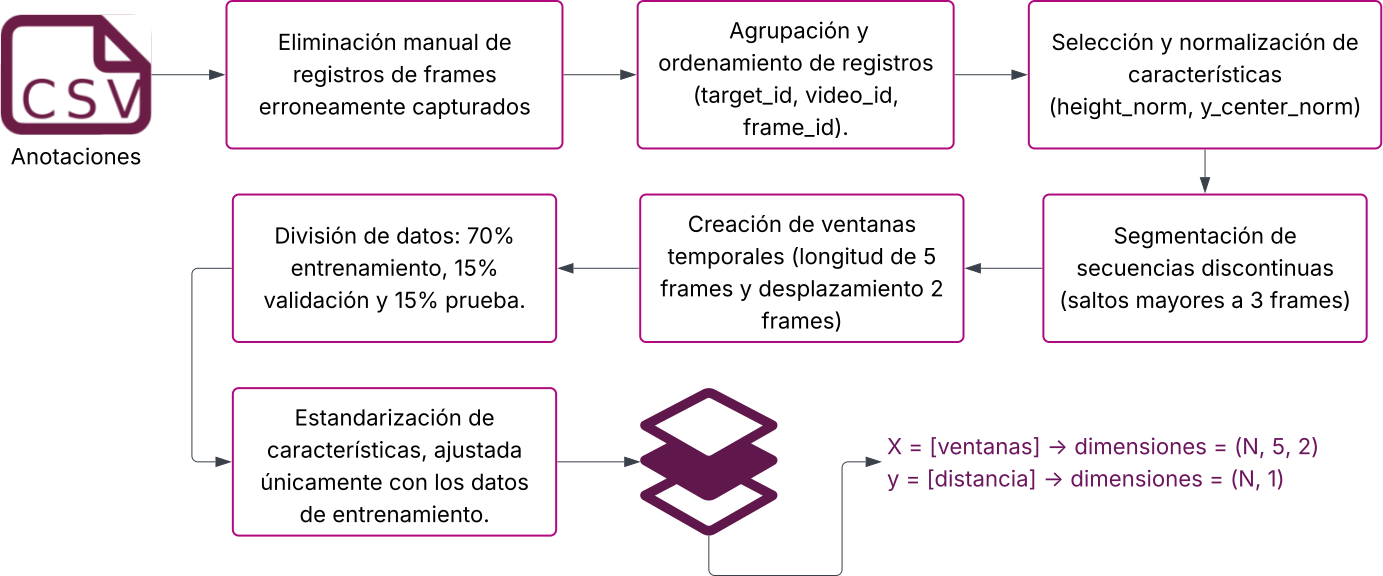
\includegraphics[width=\linewidth]{images/metodologia/preprocess_data.pdf}
    \caption{Etapas de tratamiento de las anotaciones}
    \label{fig:diag_preprocess}
\end{figure}

\subsubsection{Depuración de datos}

Durante la inspección de calidad de las anotaciones se observó que existieron errores de identificación y seguimiento provistos por el algoritmo DeepSORT (ver Fig.\ref{fig:diag_etiquetado}). Esto debido a que, ante oclusiones o cambios bruscos en la apariencia o posición, el algoritmo prioriza la asociación que minimiza su costo interno (apariencia + predicción del filtro Kalman), lo que puede conducir a confundir detecciones cercanas. Estas reasignaciones dieron lugar a distancias anotadas que no correspondían al sujeto objetivo.\\
Para detectar estos fallos se generaron versiones del video con las anotaciones (bbox, identificador de track y distancia anotada) superpuestas por cada target; esta revisión visual inicial permitió localizar y contextualizar los instantes en que las anotaciones resultaban incongruentes con la distancia conocida del sujeto.\\ 
A partir de esta referencia visual, la depuración consistió en verificar, la correspondencia entre la bbox y el sujeto de interés, revisando el historial temporal del track para detectar cambios de identidad y se contrastaron los valores de distancia anotada con la observación directa en el vídeo. Cuando la evidencia mostraba que la detección correspondía a otra persona u objeto la anotación se consideró errónea y se eliminó del conjunto de trabajo

\subsubsection{Análisis de datos}

A partir del archivo con las anotaciones ya depuradas se realizó un análisis exploratorio para justificar la selección de variables a emplear en el entrenamiento del modelo. La selección se apoyó en una matriz de correlación entre las variables anotadas y la distancia. La matriz de correlación (Figura~\ref{fig:dataCorr}) se calculó utilizando la correlación de Pearson sobre las columnas numéricas relevantes y se visualizó mediante un \emph{heatmap}.

\begin{figure}[H]
    \centering
    \includegraphics[width=\linewidth]{images/metodologia/corr.png}
    \caption{Matriz de correlación entre características geométricas y distancia}
    \label{fig:dataCorr}
\end{figure}

A partir de esta matriz se identificaron dos características con mayor correlación negativa respecto a la distancia: la altura del cuadro envolvente (bbox height, \textminus 0.84) y la coordenada vertical de su centro (y\_center, \textminus 0.30). Ambas variables se relacionan de manera inversa con la distancia real, ya que, conforme una persona se aleja de la cámara, su tamaño proyectado en la imagen disminuye y, en consecuencia, la altura del \emph{bbox} se reduce.\\
De forma complementaria, la perspectiva de la cámara provoca que el centro del objeto se desplace gradualmente hacia la parte superior del fotograma; es decir, valores menores de y\_center suelen asociarse con objetos más lejanos.\\
Para reducir multicolinealidad y favorecer que el modelo aprenda características claramente informativas, se optó por seleccionar una sola variable del grupo redundante (en este caso la altura) dado que presentó la correlación más alta con la distancia. La coordenada vertical del centro (y\_center) se conservó porque no evidenció redundancia con la altura y aporta información geométrica complementaria ligada a la perspectiva de la cámara. En consecuencia, las variables utilizadas como entradas principales del modelo fueron la altura del \emph{bbox} y la coordenada vertical del centro, decisión que además simplifica la interpretación del modelo y reduce la dimensionalidad del espacio de entrada.

\subsubsection{Segmentación temporal}
Una vez definido el conjunto depurado de anotaciones, las muestras se organizaron siguiendo una estructura jerárquica basada en el individuo registrado (\textit{target\_id}), el video correspondiente (\textit{video\_id}) y el índice temporal de cada imagen (\textit{frame\_id}). Esta organización permitió reconstruir las secuencias originales de cada persona y preservar la relación temporal entre los cuadros capturados, condición necesaria para la posterior creación de ventanas temporales. \\
Posteriormente, se verificó la continuidad temporal de cada secuencia. La depuración previa de cuadros con anotaciones inválidas podía introducir saltos abruptos en el índice de fotogramas, comprometiendo la coherencia temporal necesaria para el aprendizaje secuencial. Para corregirlo, se realizaron segmentaciones; cada video se recorrió en busca de pérdidas superiores a tres \textit{frames} consecutivos, de manera que si esto ocurre se divide la secuencia en dos diferentes, con el punto de corte justo en la posición de la pérdida de frames. Al finalizar este proceso se obtienen múltiples cadenas de frames con una correcta consistencia temporal.


A partir de las subsecuencias temporalmente consistentes obtenidas tras la segmentación, se procede a la construcción de ventanas deslizantes que constituyen las muestras de entrada para el modelo.
Cada ventana está definida por una longitud fija (\textit{seq\_len}) y un desplazamiento entre ventanas consecutivas (\textit{stride}).\\
La longitud de ventana propuesto es de diez valores, de cada secuencia original se tomarán estos cinco valores y se seleccionarán con un desplazamiento de dos frames hacia adelante. Lo anterior permite aumentar el número de muestras y mantiene la dinámica temporal de la secuencia.\\
Formalmente, para una segmento de longitud \(L\), el número de ventanas generadas se calcula como:

\begin{equation}
    N_{\text{ventanas}} = \left\lfloor \frac{L - \text{longitud\_ventana}}{\text{desplazamiento}} \right\rfloor + 1
    \label{eq:n_ventanas}
\end{equation}

En la figura \ref{fig:windowsGen} se ilustra la cantidad de ventanas generadas por target dada la ecuación \ref{eq:n_ventanas}.

\begin{figure}[H]
    \centering
    \includegraphics[width=\linewidth]{images/metodologia/frames-ventanas.png}
    \caption{Número de ventanas generadas por individuo-video}
    \label{fig:windowsGen}
\end{figure}

\subsubsection{Partición del conjunto de datos}
Con las ventanas generadas por individuo, se procede a la partición del conjunto de datos en subconjuntos de entrenamiento (\emph{train}), validación (\emph{val}) y prueba (\emph{test}).\\
Antes de aplicar la partición, se definió manual y deliberadamente qué \emph{targets} pertenecerían a cada subconjunto; esta asignación buscó favorecer la capacidad de generalización del modelo, procurando que \emph{train}, \emph{val} y \emph{test} incluyeran individuos con distinta variabilidad (por ejemplo, rangos de estatura y condiciones de captura diversas), siempre garantizando que ningún \emph{target} se repita entre subconjuntos.\\
A partir de las listas manuales, la separación efectiva se llevó a cabo mediante máscaras booleanas: para cada ventana se comprueba si su \emph{target\_id} aparece en la lista correspondiente, generando filtros que seleccionan todas las ventanas asociadas a los individuos asignados. Este mecanismo asegura que cada persona quede íntegramente contenida en un único subconjunto, evita fugas de información entre entrenamiento y evaluación y contribuye a que el rendimiento reportado refleje de manera más fiel la capacidad de extrapolación del modelo.\\
\begin{figure}[H]
    \centering
    % Subfigura lateral derecho
    \begin{subfigure}{0.45\textwidth}
        \centering
        \includegraphics[width=\linewidth]{images/resultados/pastel_tvt.png} \\
        \caption{Porcentajes por subgrupo}
        \label{subfig:cake-tvt}
    \end{subfigure}
    \hfill
    % Subfigura central
    \begin{subfigure}{0.45\textwidth}
        \centering
        \includegraphics[width=\linewidth]{images/resultados/distancias-por-grupo.png} \\
        \caption{Distribución de distancias por subgrupo}
        \label{subfig:distances-tvt}
    \end{subfigure}
    \caption{Distribución de los subgrupos de entrenamiento, prueba y validación}
    \label{fig:result_distr_tvt}
\end{figure}
La proporción resultante entre los subgrupos y la cobertura de los rangos de distancia en cada subconjunto se ilustran en la Figura \ref{fig:result_distr_tvt}, lo que permite verificar empíricamente tanto el balance de tamaños como la representatividad de las distancias.

\subsubsection{Normalización de características}
La normalización se realizó después de la partición en \emph{train}, \emph{val} y \emph{test} descrita en la sección previa, empleando el escalado Min--Max calculado exclusivamente sobre los datos de entrenamiento. 
Esta elección responde a la necesidad de conservar la distribución relativa de las dimensiones geométricas extraídas del \emph{bbox} y a la ventaja práctica de producir valores dentro de un rango acotado [0,1], lo que suele acelerar la convergencia y estabilizar el entrenamiento. Así mismo, al estimar los parámetros únicamente sobre \emph{train} se evita una fuga de información hacia los subconjuntos de validación y prueba, previniendo sesgos optimistas en la evaluación.

Formalmente, denotando por \emph{x} una componente cualquiera de las características, el escalado aplicado es:

\begin{equation}
x' = \frac{x - x_{\min}}{x_{\max} - x_{\min} + \varepsilon},
\label{eq:minmax}
\end{equation}
Donde \(\,x_{\min}\,\) y \(\,x_{\max}\,\) son el mínimo y el máximo de la característica calculados sobre todos los fotogramas contenidos en las ventanas del conjunto de entrenamiento, y \(\,\varepsilon\,\) es una constante pequeña \((\varepsilon = 10^{-8})\) para evitar divisiones por cero cuando \(x_{\min} = x_{\max}\).


\subsection{Entrenamiento del modelo recurrente}
En esta etapa se implementa y compara una arquitectura basada en LSTM y otra basada en GRU, ambas orientadas a la tarea de regresión de la distancia en metros a partir de las secuencias temporales generadas y de las características geométricas seleccionadas tras el análisis de correlación. A lo largo de la sección se describirá la estrategia de agrupación en lotes (\emph{batching}), la arquitectura de cada red, los hiperparámetros de entrenamiento y las métricas empleadas para la evaluación.
\subsubsection{Procesamiento por lotes}
Dada la naturaleza secuencial de las muestras, la estrategia de agrupación en lotes (\emph{batching}) se diseñó para preservar la coherencia temporal y evitar la mezcla de ventanas de distintos individuos dentro del mismo lote (\emph{batch}). Para ello se emplea una clase de generación de lotes (\emph{batches}) que agrupa las ventanas por \emph{target\_id} (cada batch contiene únicamente ventanas pertenecientes al mismo individuo). Este procedimiento facilita el aprendizaje de dinámicas temporales coherentes y permite controlar explícitamente el barajado a nivel de batches —barajado activo en entrenamiento y desactivado en validación—, contribuyendo a una evaluación más estable y representativa.

\subsubsection{Configuración de entrenamiento y definición de hiperparámetros}
La configuración de entrenamiento se definió de forma común para las dos variantes de arquitecturas (LSTM y GRU). En ella se establecen los criterios y parámetros que se mantendrán idénticos para permitir comparaciones controladas y reproducibles. \\
El procedimiento de entrenamiento inicia con la carga de las secuencias de entrenamiento y validación, junto con sus etiquetas de distancia y los identificadores de individuo necesarios para la generación de los lotes. Estas secuencias se organizan mediante el esquema de batching descrito previamente: los lotes se mantienen homogéneos por \emph{target\_id} y sólo se barajan en el conjunto de entrenamiento. \\
Una vez generados los lotes, se instancia el modelo recurrente correspondiente (LSTM o GRU) mediante una función constructora que recibe como parámetros la longitud de secuencia y el número de características. De esta forma, la estructura del entrenamiento permanece fija y únicamente la arquitectura interna del bloque recurrente varía entre experimentos.\\
Para controlar el proceso de entrenamiento se emplean callbacks estándar pero afinados para el problema de regresión en distancia:
\begin{itemize}
  \item \raggedright \textbf{EarlyStopping} monitorizando \texttt{val\_mae} y recuperando los mejores pesos mediante \texttt{restore\_best\_weights}, con el fin de detener el entrenamiento cuando no se observe mejora y evitar sobreajuste.
  \item \textbf{ReduceLROnPlateau} monitorizando \texttt{val\_mae}, para disminuir la tasa de aprendizaje cuando el progreso en validación se estabiliza.  
  \item \textbf{ModelCheckpoint} para guardar el mejor modelo (formato \texttt{.keras}) durante el entrenamiento.
  \item \textbf{CSVLogger} para conservar un registro de las métricas por época y facilitar análisis posteriores.
\end{itemize}

A modo de referencia, la configuración experimental de hiperparámetros usada en el presente trabajo se resume en la Tabla \ref{tab:hiperparametros_entrenamiento}.
\begin{table}[H]
\centering
\begin{tabular}{ll}
\hline
Parámetro & Valor (por defecto) \\
\hline
Optimizer & Adam \\
Learning rate inicial & $1\times 10^{-4}$ \\
Loss & MSE \\
Métrica principal & MAE \\
Epochs máximas & 200 \\
Batch size (seq. por batch) & 32 \\
EarlyStopping (monitor) & val\_mae, patience=30, min\_delta=0.01 \\
ReduceLROnPlateau & factor=0.5, patience=15, min\_lr=1e-7 \\
ModelCheckpoint & guarda mejor val\_mae (.keras) \\
CSVLogger & registra por-época training\_log.csv \\
\hline
\end{tabular}
\caption{Hiperparámetros de entrenamiento.}
\label{tab:hiperparametros_entrenamiento}
\end{table}

\subsubsection{Arquitectura GRU}
La variante GRU utilizada en este trabajo intenta equilibrar capacidad de modelado temporal y simplicidad operativa. Dada la entrada temporal estructurada en ventanas y compuesta por dos variables por paso (las características geométricas seleccionadas durante el análisis); el procesamiento de dichas ventanas y el batching por \emph{target\_id} siguen el procedimiento descrito previamente en la sección de preprocesamiento y se ilustran de manera general en la Figura \ref{fig:gru_rnn}.
\begin{figure}[H]
    \centering
    \includegraphics[width=\linewidth]{images/metodologia/rnnGru.png}
    \caption{Arquitectura de la RNN basada en GRU}
    \label{fig:gru_rnn}
\end{figure}
A partir de esa entrada, la red dispone de un único bloque recurrente GRU (en la implementación experimental con 128 unidades) que resume la dinámica temporal de cada ventana en un vector de estado final para obtener una representación compacta por ventana.\\
La salida del bloque recurrente se proyecta a través de una capa densa intermedia de 64 unidades con activación ReLU, que aporta no linealidad y facilita la transformación de la representación temporal a un espacio más adecuado para la regresión. Tras esa capa densa se aplica regularización por \texttt{dropout} (en la configuración usada se fijó en 0.2) para mitigar el sobreajuste.\\
Finalmente, la capa de salida consiste en una única neurona con activación lineal que produce la predicción continua de la distancia en metros, decisión coherente con el objetivo de regresión.

\subsubsection{Arquitectura LSTM}
La variante basada en LSTM parte de la misma estructura de entrada —ventanas temporales con dos características por paso— cuyo procesamiento y agrupamiento por \emph{target\_id} siguen exactamente el flujo de batching descrito; el esquema de la arquitectura se muestra en la Figura \ref{fig:rnnlstm}.
\begin{figure}[H]
    \centering
    \includegraphics[width=\linewidth]{images/metodologia/rnnLSTM.png}
    \caption{Arquitectura de la RNN basada en LSTM}
    \label{fig:rnnlstm}
\end{figure}
A continuación, la secuencia entra a una única capa LSTM de 32 unidades (con \texttt{return\_sequences=False}), cuyo estado final resume la dinámica temporal de la ventana. La elección de un número reducido de unidades —en contraste con las 128 usadas en la variante GRU— se debe a que las LSTM tienen una estructura interna más compleja y costosa (compuertas y estado de celda), por lo que incrementar su dimensionalidad eleva significativamente el coste computacional. Al igual que en la arquitectura previa, se aplica regularización mediante \emph{dropout} (configurado en 0.1) tanto en las conexiones de entrada como en las recurrentes con el fin de mitigar sobreajuste sin incrementar la complejidad del modelo. \\
La representación generada por el LSTM se proyecta finalmente a una capa densa de 16 unidades con activación \texttt{relu}, que actúa como transformación no lineal previa a la estimación. La salida corresponde a una única neurona lineal, para producir el valor continuo de distancia que el modelo debe predecir.
